\subsection*{Træning} \label{sec:traening}
Inden brugeren kan træne skal træningen tilpasses den enkelte bruger. Tilpasning af træningsniveauet er  yderligere beskrevet af \autoref{fig:traeningsniveau}.
Aktivitetsdiagrammet over træningen fremgår af \autoref{fig:traening}. 

\begin{figure} [H]
\centering
\textbf{Aktivitetsdiagram: Træning}\par\medskip
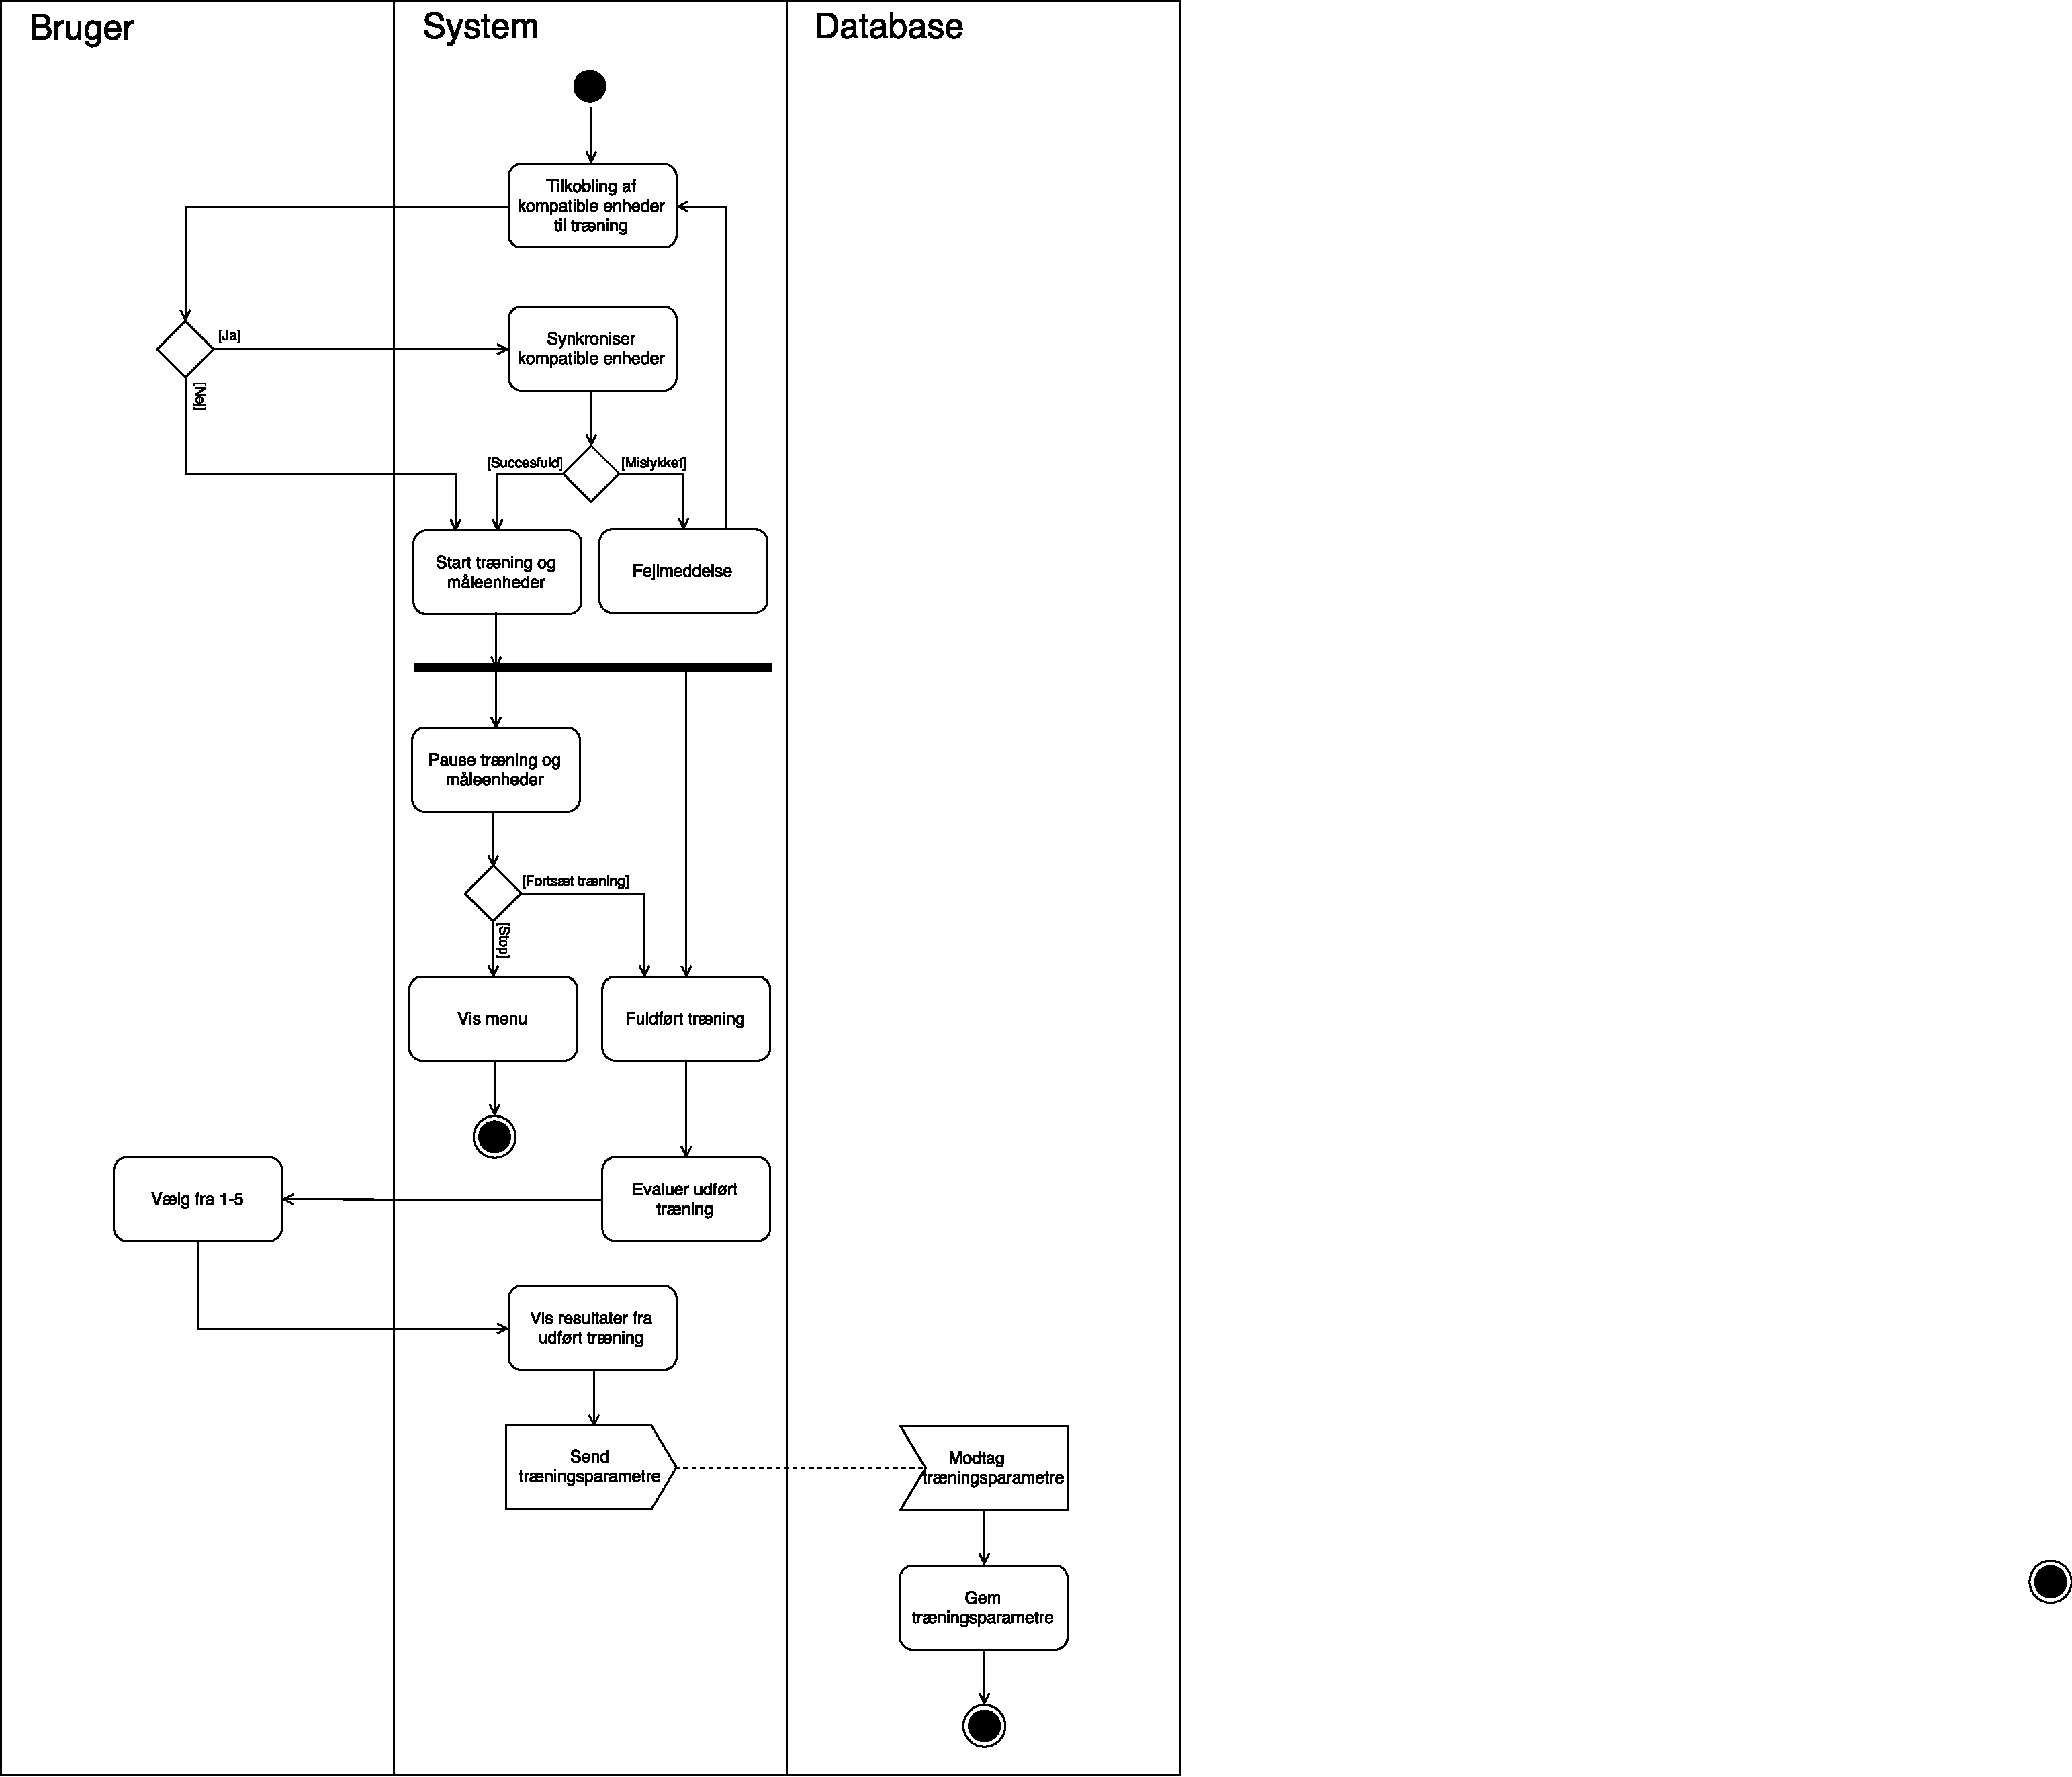
\includegraphics[width=1\textwidth]{figures/aktivitetsdiagram/Traening}
\caption{Aktivitetsdiagram over træning. Tilpasning af træningsniveau uddybes af \autoref{fig:traeningsniveau}.}
\label{fig:traening}
\end{figure}

\noindent
Når systemet har tilpasset træning vises grænsefladen for træning. Brugeren kan påbegynde træningen ved at trykke start, hvorefter timer og GPS starter. Under træningen vil tid og afstand kontinuert fremgå af grænsefladen. Brugeren kan til en hver tid vælge at afslutte træningen ved at trykke på stop træningen, hvilket medfører, at timer og GPS stoppes og grænsefladen for afslut træning vises. Denne handling skal bekræftes i tilfælde af, at brugeren ved en fejl angiver, at træningen skal stoppes. Ved en fejl vises grænsefladen for træning. Ved bekræftelse af stop træning, vises grænsefladen for evaluering af udført træning, hvor brugeren skal angive en evaluering. Efterfølgende sendes evalueringen og træningsresultater til en database, hvor det gemmes.


\subsubsection*{Tilpasning af træningsniveau} \label{sec:traeningsniveau}
Før selve træningen påbegyndes, skal træningsniveauet tilpasses brugeren. 

Tilpasning af træningsniveau er en funktion der skal tage højde for daglige variationer ved at anbefale et træningsniveau ud fra brugeres kategorisering, daglige helbredstilstand og tidligere evalueringer af træninger.  
Aktivitetsdiagrammet over tilpasning af træningsniveau fremgår af \autoref{fig:traening}.

\begin{figure} [H]
\centering
\textbf{Aktivitetsdiagram: Tilpasning af træning}\par\medskip
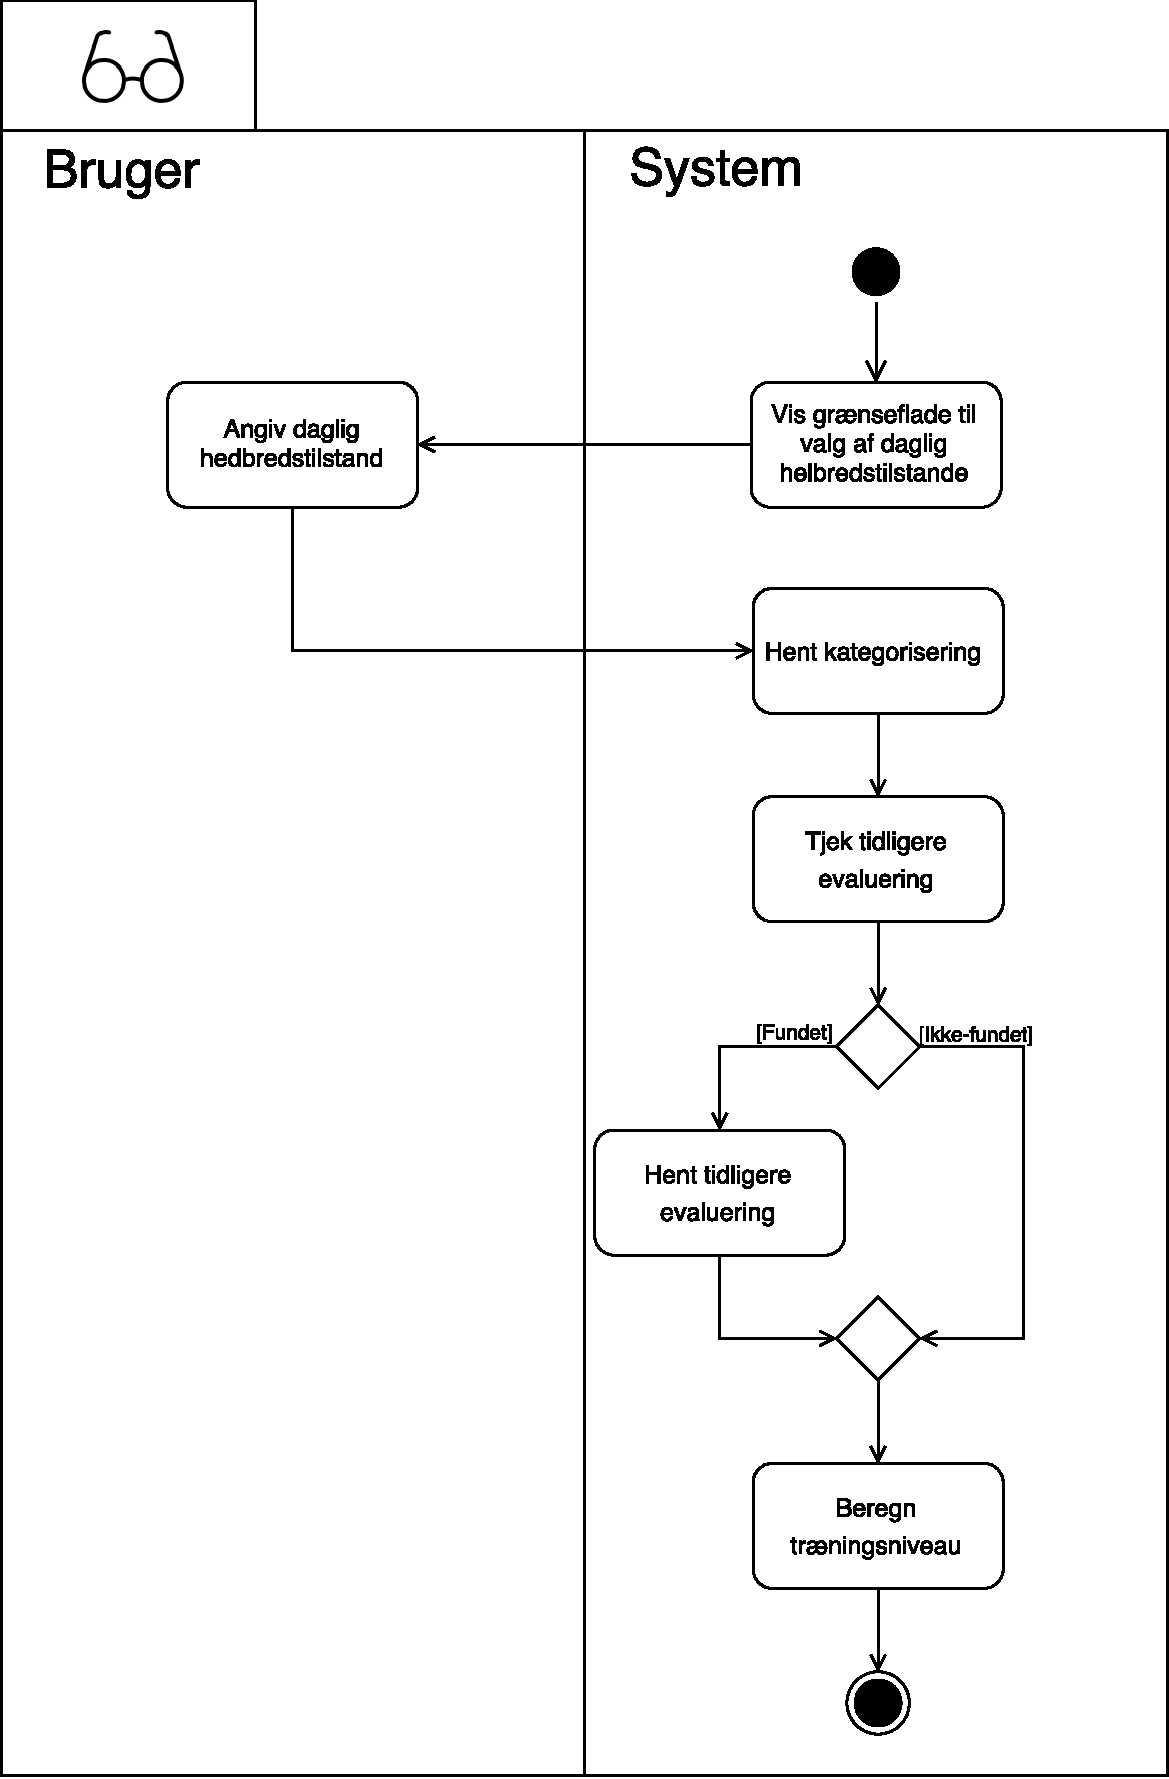
\includegraphics[width=0.9\textwidth]{figures/aktivitetsdiagram/Tilpasningaftraeningsniveau}
\caption{Aktivitetsdiagram over tilpasning af træningsniveau.}
\label{fig:traeningsniveau}
\end{figure}

\noindent
Systemet viser grænsefladen for valg af træningsform, hvor brugeren skal angive den ønskede træningsform, herunder konditions-, styrketræning eller vejrtrækningsøvelser. Ud fra den valgte træningsform skal brugeren angive træningstype, eksempelvis kan der ved valg af konditionstræning vælges gå, løbe eller cykle. Herefter vises grænsefladen for valg af daglig helbredstilstande, hvortil brugeren skal angive sin helbredstilstand. Systemet henter kategorisering, hvorefter den anmoder om tidligere evaluering i databasen. Databasen tjekker om der er tidligere evalueringer for den valgte træningsform og -type. Hvis brugeren ikke har angivet tidligere evalueringer bestemmes niveauet ud fra de resterende parametre. Hvis der findes tidligere evalueringer hentes disse og medregnes som en parameter.  Et simpel eksempel på denne beregning fremgår af \autoref{tab:beslutningstabel}. Tabellen beskriver, hvordan en algoritme vil kunne regulere træningsniveauet, således der tages højde for den enkelte bruger.

\begin{table}[H]
\centering
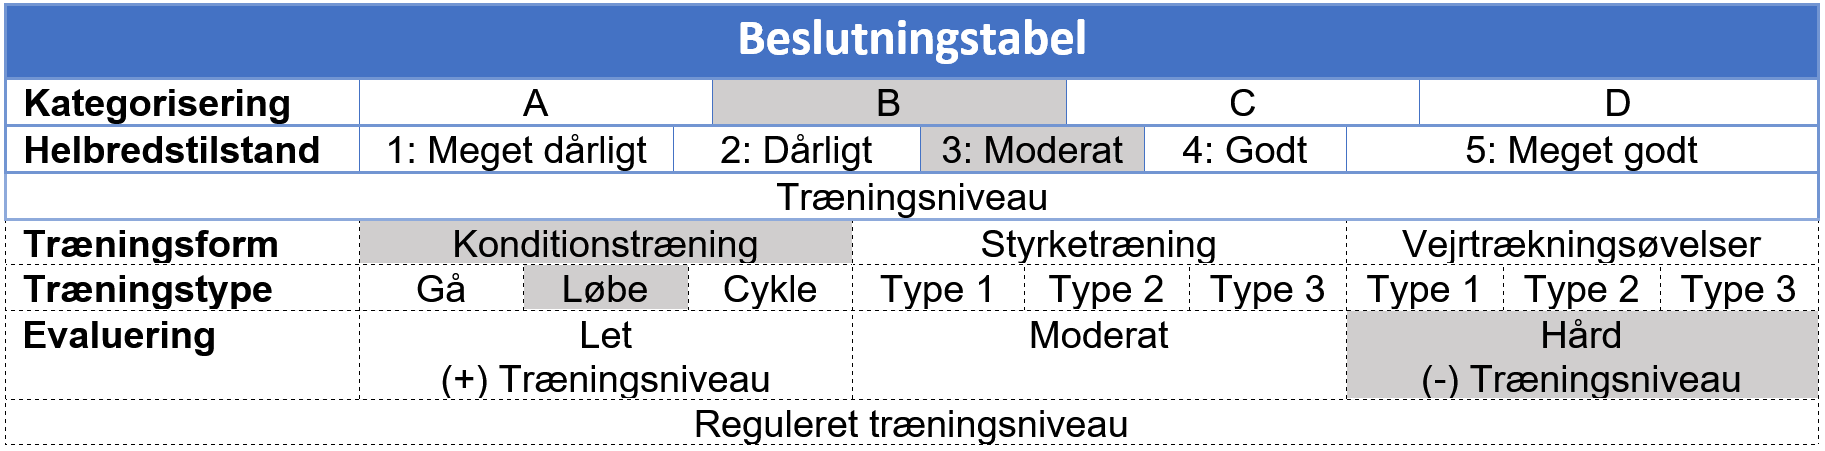
\includegraphics[width=1\textwidth]{figures/aktivitetsdiagram/beslutningstabel}
\caption{Beslutningstabel for træningsniveau. Kategorisering, daglig helbredstilsand samt eventuel evaluering anvendes til at bestemme træningsniveauet til den enkelte bruger. Af dette eksempel er brugeren kategoriseret B, har valgt konditionstræning, herunder løb. Derudover har brugeren angivet sin helbredstilstand til moderat. Ud fra dette kan der tilpasset et træningsniveau. Hvis brugeren tidligere har evalueret en træningen inden for konditræning og løb anvendes denne evaluering til regulere træningsniveauet. I dette tilfælde har brugeren tidligere evalueret træningen til hård, hvorfor niveauet af træningen sænkes.}
\label{tab:beslutningstabel}
\end{table} 

\noindent
Af \autoref{tab:beslutningstabel} fremgår en simpel beslutningstabel for, hvorledes et træningsniveau tilpasses den enkelte bruger. Beslutningstabellen tager udgangspunkt i brugerens kategorisering, valgt træningsform og -type samt daglig helbredstilstand og en eventuel evaluering. Brugeren er i dette tilfælde kategoriseret til B. Valgt at udføre konditionstræning herunder løb. Helbredstilstanden angives førend en træning påbegyndes, for således at tilpasse niveauet til den pågældende dag. Helbredstilstanden angives efter \textit{1: Meget dårligt}, \textit{2: Dåligt}, \textit{3: Moderat}, \textit{4: Godt} eller \textit{5: Meget godt}, hvortil brugerens helbredstilstand her angives som moderat.
Træningsniveauet vurderes dermed ud fra brugerens kategorisering, valg af træningsform og -type samt helbredstilstand. 
For at have mulighed for at kunne regulere træningsniveauet yderligere, medregnes den forhenværende evaluering, der er forbundet med samme helbredstilstand, træningsform og type. I dette tilfælde har brugeren før haft samme helbredstilstand, træningsform samt -type og dertil evalueres denne træning til værende hård. Algoritmen regulerer hertil træningsniveauet for denne træning ned, for således at give brugeren en bedre og mere tilpasset træningsoplevelse. 
